%\section{问题一的模型建立与求解}
%
%\subsection{数据预处理}
%
%采用 Z-score 标准化处理：$x' = \frac{x - \mu}{\sigma}$。
%
%\subsection{模型建立}
%
%问题一包含GPU需求短期预测与基础算力调度两个相互独立的任务。
%预测部分利用第0--2375小时历史工作负载预测第2376--2399小时GPU需求；
%调度部分则直接使用第2376--2399小时实际到达任务，
%预测结果仅用于预测精度评价，不参与任务调度。
%
%首先按照“区域--任务类型--小时”统计GPU到达需求。
%设区域$r$、任务类型$k$在时刻$t$的新到达GPU需求为$D_{rkt}$，
%则有
%\begin{equation}
%	D_{rkt}
%	=
%	\sum_{\substack{i:\,ArrivalHour_i=t\\
%			SourceRegion_i=r,\;TaskType_i=k}}
%	GPU\_Demand_i .
%\end{equation}
%
%由此得到$6\times3=18$条底层需求序列。
%考虑到细粒度序列存在较多零值和随机尖峰，
%进一步构造区域需求$D_{rt}=\sum_kD_{rkt}$、
%任务类型需求$D_{kt}=\sum_rD_{rkt}$以及系统总需求
%$D_t=\sum_rD_{rt}$。
%其中18条底层序列用于刻画区域与任务类型异质性，
%而稳定性较高的区域层、任务类型层和系统层序列用于短期预测。
%
%对于任一聚合需求序列$y_t$，
%利用预测时点之前最近$H$小时的局部平均需求水平预测未来24小时，
%即
%\begin{equation}
%	\hat{y}_{T+h}(H)
%	=
%	\frac{1}{H}
%	\sum_{\tau=T-H+1}^{T}y_{\tau},
%	\qquad h=1,2,\ldots,24 .
%\end{equation}
%
%式(2)中，$T$为预测起点前最后一个已知时刻，
%$H$为历史窗口长度。
%在$H\in\{24,72,168,336\}$中，
%利用第2352--2375小时验证集选择预测窗口，
%模型确定后再使用第0--2375小时历史信息重新估计局部需求水平，
%对第2376--2399小时进行最终预测。
%该过程严格保持时间前向性，测试期真实数据不参与模型选择。
%
%由于区域需求、任务类型需求和系统需求分别预测后可能出现总量不一致，
%首先以系统总需求预测作为逐时总量锚点，
%对区域预测和任务类型预测进行比例调整，
%使二者的逐时总和均与系统预测一致。
%随后利用历史区域--任务类型需求结构$q_{rk}$恢复18类交叉需求。
%设恢复后的需求为$z_{rkt}$，则其满足
%\begin{equation}
%	\begin{aligned}
%		\min_{z_{rkt}\geq 0}\quad
%		&\sum_r\sum_k
%		z_{rkt}\ln\frac{z_{rkt}}{q_{rk}},\\
%		\mathrm{s.t.}\quad
%		&\sum_k z_{rkt}=\tilde{D}_{rt},\\
%		&\sum_r z_{rkt}=\tilde{D}_{kt}.
%	\end{aligned}
%\end{equation}
%
%其中，$\tilde{D}_{rt}$和$\tilde{D}_{kt}$分别表示一致性调整后的区域需求和任务类型需求。
%式(3)在保持两个边际预测结果不变的条件下，
%使恢复后的18类需求尽可能接近历史业务结构，
%从而兼顾细粒度需求解释能力与预测稳定性。
%预测效果采用WAPE、RMSE和MAE进行评价，
%并与24小时前同一时刻的需求作为基准进行比较。
%
%在基础算力调度中，设任务$i$的GPU需求为$g_i$，
%持续时间为$d_i$，
%来源区域为$r_i^0$。
%根据任务最大允许网络时延预先确定候选执行区域集合$R_i$。
%实时推理任务到达后立即开工；
%批量推理和AI训练任务则在最早开工时间、最晚完成时间以及2406终端边界内确定候选开工时刻集合$S_i$。
%定义二元变量$x_{irs}$表示任务$i$是否在区域$r$、时刻$s$开始执行，
%每个任务只能选择唯一的执行区域和开工时刻。
%
%由于任务持续时间以分钟给出，而资源容量按小时统计，
%不能将跨小时任务简单视为完整占用每个小时。
%任务$i$在时刻$s$开工后与小时区间$[t,t+1)$的实际重叠比例定义为
%\begin{equation}
%	\rho_{ist}
%	=
%	\max\left\{
%	0,\,
%	\min(s+d_i,t+1)-\max(s,t)
%	\right\}.
%\end{equation}
%
%式(4)使分钟级任务能够准确映射到逐小时GPU和功率占用。
%设任务$i$完整运行时的AI IT功率为
%$p_i=g_iP^{GPU}_{k(i)}$，
%其中$P^{GPU}_{k(i)}$为对应任务类型的单位GPU功率。
%同时记区域$r$在时刻$t$可供AI任务使用的有效IT功率为
%$A_{rt}$，其由最大IT功率、设施功率、PUE以及非AI固定负荷共同确定。
%基础调度需要满足以下主要资源约束：
%\begin{equation}
%	\begin{aligned}
%		&\sum_{r\in R_i}\sum_{s\in S_i}x_{irs}=1,
%		&&\forall i,\\
%		&\sum_i\sum_{s\in S_i}
%		g_i\rho_{ist}x_{irs}
%		\leq AvailableGPU_r,
%		&&\forall r,t,\\
%		&\sum_i\sum_{s\in S_i}
%		p_i\rho_{ist}x_{irs}
%		\leq A_{rt},
%		&&\forall r,t .
%	\end{aligned}
%\end{equation}
%
%第一项保证每个任务唯一执行；
%第二项限制各区域逐时GPU占用不超过可调度GPU容量；
%第三项同时控制IT功率与经PUE折算后的设施功率边界。
%此外，候选集合$R_i$和$S_i$已经预先排除了违反网络时延、
%最早开工时间、最晚完成时间及2406终端要求的组合，
%从而保证生成的任务安排满足基本服务约束。
%
%问题一尚未引入电价、碳排放、新能源和储能因素，
%因此将其作为后续算电协同调度的中性算力基线。
%首先最小化跨区域迁移的GPU工作量，
%在一级目标达到最优后固定其最优值，
%再最小化弹性任务累计等待时间：
%\begin{equation}
%	\begin{aligned}
%		\min\quad
%		F_1
%		&=
%		\sum_i
%		\sum_{\substack{r\in R_i\\r\neq r_i^0}}
%		\sum_{s\in S_i}
%		g_i d_i x_{irs},\\
%		\text{在 }F_1=F_1^{*}\text{ 条件下，}\qquad
%		\min\quad
%		F_2
%		&=
%		\sum_{i\in I^{\mathrm{flex}}}
%		\sum_{r\in R_i}\sum_{s\in S_i}
%		(s-EarliestStart_i)x_{irs}.
%	\end{aligned}
%\end{equation}
%
%式(6)形成“优先减少不必要的跨区域迁移，其次减少弹性任务等待”的两级调度目标。
%其中采用$g_id_i$衡量迁移GPU工作量，
%能够同时反映任务规模和运行持续时间，
%避免将小型短时任务与大型长时训练任务等同处理。
%最终根据调度结果计算各区域逐时GPU利用率，
%并形成第2376--2405小时的任务执行过程，
%以完整展示第2376--2399小时到达任务及其收尾情况。
%
%
%
%
%\subsection{求解结果与模型检验}
%
%
%预测部分首先在候选历史窗口$H\in\{24,72,168,336\}$中，
%利用第2352--2375小时验证集选择式(2)中的窗口长度。
%验证结果表明，$H=72$时总体WAPE最低，因此将72小时作为最终历史窗口；
%随后使用第0--2375小时数据重新估计区域、任务类型和系统层的局部需求水平，
%并对第2376--2399小时进行24小时预测。
%在此基础上，根据式(3)进行层级一致性恢复，
%得到完整的18类“区域--任务类型”GPU需求预测结果。
%
%从需求结构看，不同区域和任务类型之间存在明显异质性。
%如图1所示，18类GPU需求在小时尺度上均伴随一定随机波动和间歇性尖峰，
%其中RegionD、RegionE和RegionF的AI训练需求长期处于较高水平，
%累计GPU需求分别达到407683、292000和296143，
%明显高于RegionA、RegionB和RegionC对应的63070、62551和58899；
%实时推理需求则更多集中于东部区域。
%这说明任务类型与空间位置具有明显关联，
%若直接对18条细粒度序列分别进行预测，
%容易受到随机到达和极端任务的影响。
%
%% ==================== 图1 ====================
%% width控制图片宽度：
%% 0.85\textwidth 表示占正文宽度的85%，如感觉过大可改为0.75或0.8
%% [htbp]控制浮动位置：h=当前位置，t=页顶，b=页底，p=浮动页
%% 若希望尽量放在当前位置，可使用[H]，但需要导言区加入 \usepackage{float}
%\begin{figure}[H]
%	\centering
%	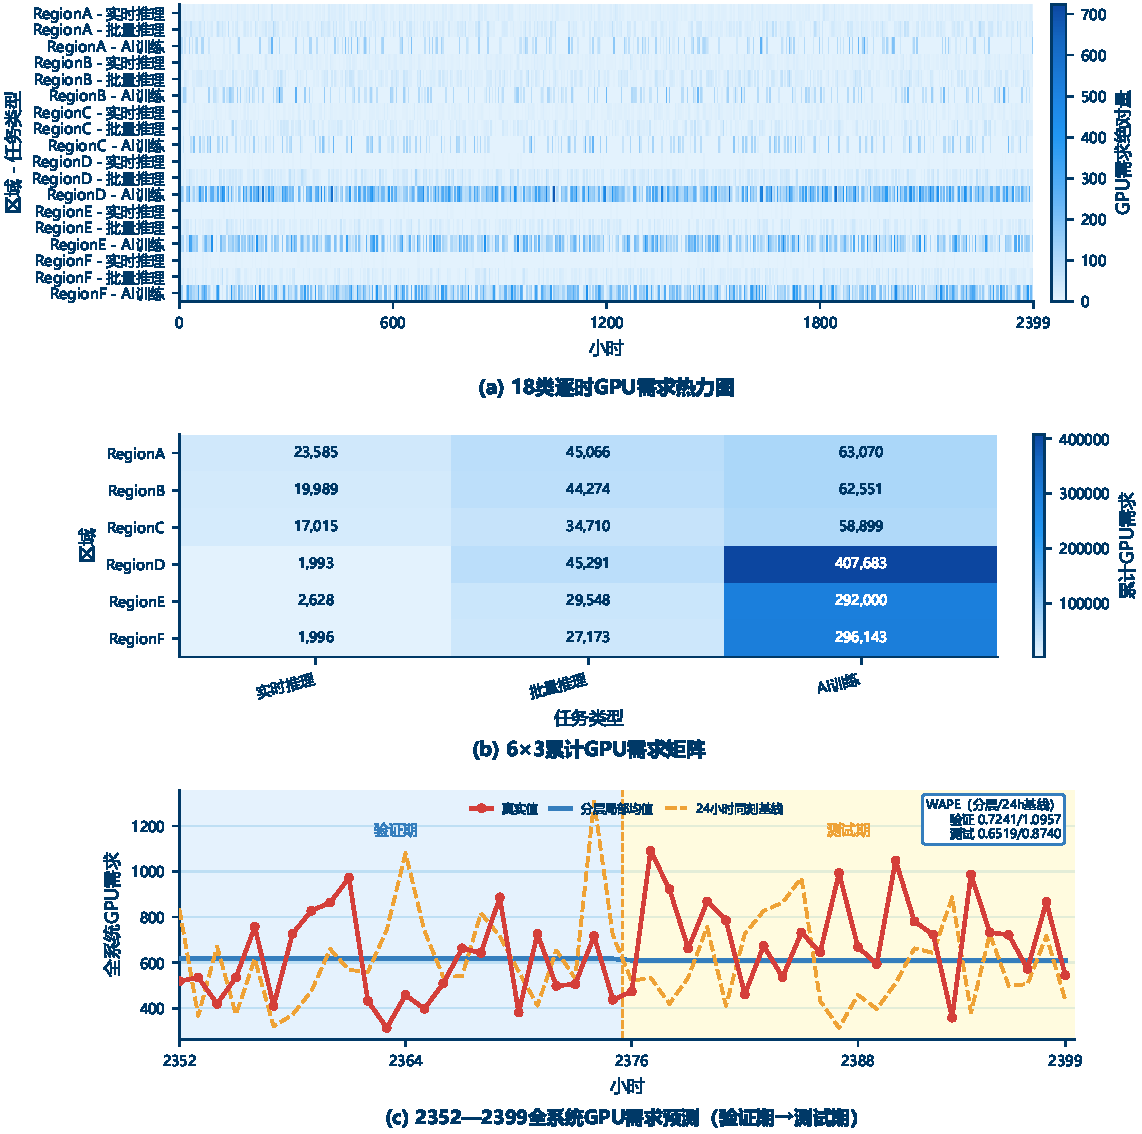
\includegraphics[width=0.88\textwidth]{figures/q1_group1_demand_structure.pdf}
%	\caption{GPU需求异质性与分层短期预测结果}
%\end{figure}
%% =================================================
%
%图1(c)进一步给出了预测结果。
%在验证期，第2352--2375小时的分层局部均值预测
%WAPE、RMSE和MAE分别为0.7241、45.7417和23.6915，
%而24小时同刻基线分别为1.0957、69.9249和35.8495；
%在测试期，第2376--2399小时对应三项指标分别为
%0.6519、53.4704和26.3323，
%基线则为0.8740、72.8628和35.3032。
%因此，在当前验证和测试划分下，
%分层局部均值模型在三项误差指标上均优于24小时同刻基线。
%从图中也可以看到，该预测更侧重于捕捉未来24小时的局部需求水平，
%而不是强行追踪难以重复的单小时尖峰。
%因此，其主要作用是稳定刻画短期总体需求水平，
%而非精确复现每一个随机峰值。
%
%完成预测后，基础算力调度直接读取第2376--2399小时实际到达的538个任务，
%预测值不参与任务安排。
%调度按照式(6)的两级目标进行：首先最小化跨区域迁移GPU工作量，
%随后在一级目标最优的条件下最小化弹性任务等待时间。
%任务实际执行过程中根据式(4)计算跨小时重叠比例，
%并结合式(5)检查GPU容量、IT功率和设施功率约束。
%
%求解结果表明，一级目标达到
%$F_1^*=0\ \mathrm{GPU\cdot h}$，
%538个任务均可在来源区域完成，本地执行率为100\%；
%在保持零迁移的条件下，二级目标得到
%$F_2^*=3\ \mathrm{h}$。
%这意味着在问题一尚未考虑电价、碳强度和新能源条件时，
%当前算力容量本身并不会迫使任务进行跨区域迁移。
%因此，后续问题二若出现任务迁移，其主要驱动力应来自能源侧条件变化，
%而不是问题一阶段的资源不可行。
%
%% ==================== 图2 ====================
%% 若整图内容较密，建议宽度用0.90--0.95\textwidth
%% 如果图片在页面上显得太高，可改为：
%% \includegraphics[width=0.90\textwidth,height=0.78\textheight,keepaspectratio]{...}
%\begin{figure}[H]
%	\centering
%	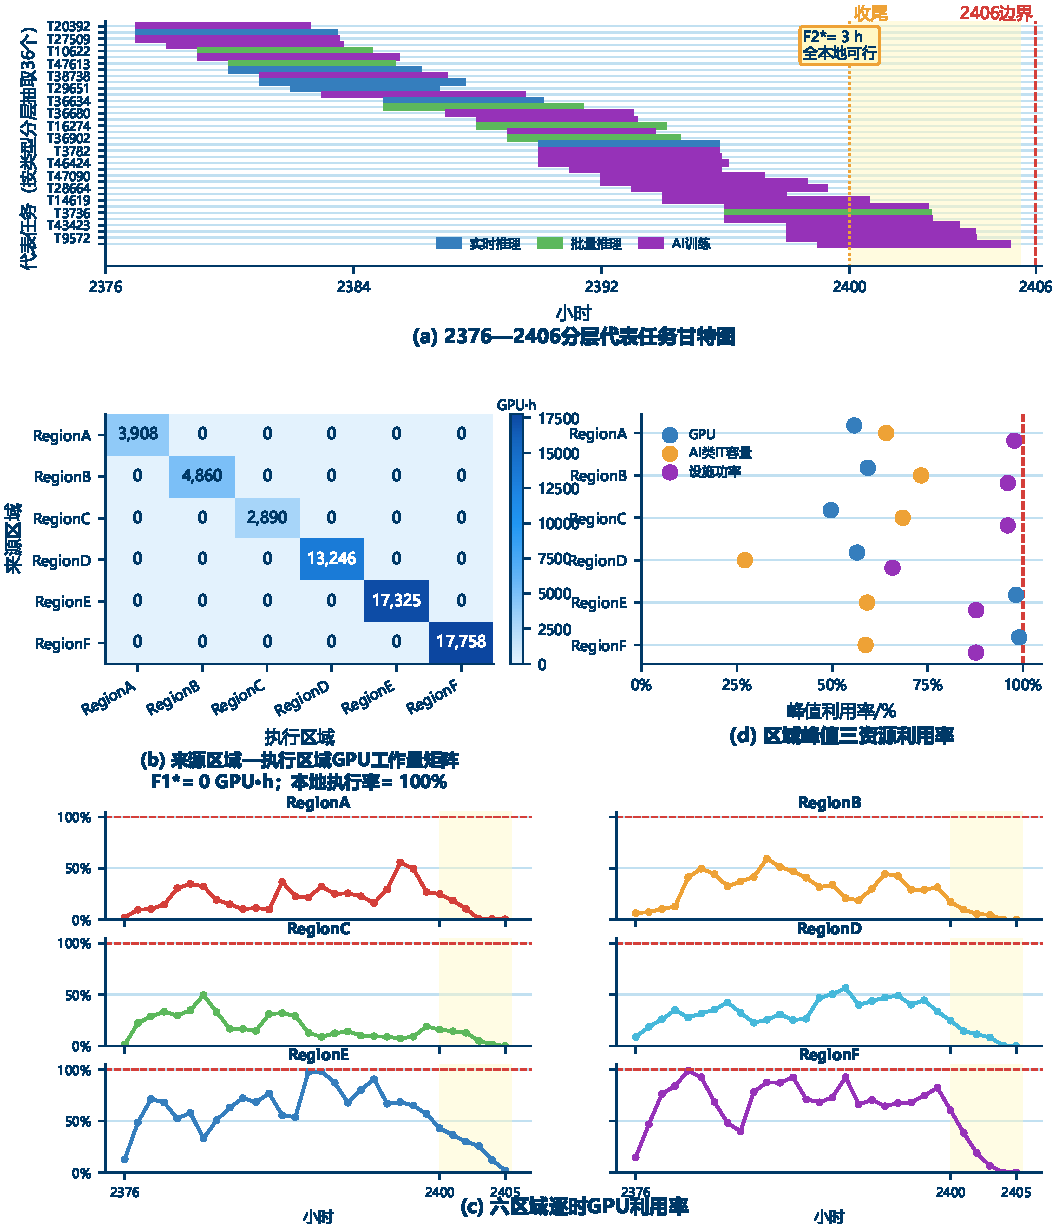
\includegraphics[width=0.92\textwidth]{figures/q1_group2_core_results.pdf}
%	\caption{基础算力调度方案与多资源承载状态}
%\end{figure}
%% =================================================
%
%图2从任务调度和资源利用两个角度进一步说明了该结果。
%代表任务甘特图显示，部分在主时域末端到达的批量推理和AI训练任务
%延伸至第2400--2405小时收尾区间，
%但所有任务均在2406边界前完成。
%来源区域--执行区域GPU工作量矩阵全部集中在主对角线上，
%与$F_1^*=0$和100\%本地执行率一致。
%
%六个区域的逐时GPU利用率进一步表明，
%不同区域的资源紧张程度并不相同。
%RegionE和RegionF在部分时段的GPU利用率接近容量上界，
%而部分东部区域虽然GPU仍有剩余，
%其设施功率利用率却已处于较高水平；
%RegionD则表现出相对充足的综合承载空间。
%因此，区域可调度能力不能仅依据GPU数量判断，
%GPU容量、AI IT功率和设施功率均可能成为实际瓶颈。
%这一结果也验证了式(5)中保留多层资源约束的必要性。
%
%为进一步检验预测结论是否依赖单一验证区间，
%对分层预测进行了84个滚动样本外窗口检验。
%如图3(a)所示，
%84个窗口中“分层模型WAPE减去24小时同刻基线WAPE”的差值全部小于0，
%即84个窗口均由分层模型取得更低WAPE，
%单侧统计检验得到$p=8.55\times10^{-16}$。
%这表明图1中观察到的预测优势并非由单一预测起点偶然产生，
%而是在不同样本外窗口中保持较稳定的一致性。
%
%同时，为检验式(3)的层级一致性恢复是否以牺牲预测精度为代价，
%将恢复后的18类需求与直接预测结果进行比较。
%图3(b)中二者WAPE中位差仅为
%$-3.05\times10^{-4}$，对应$p=0.216$，
%未观察到统计上明显的精度差异。
%另一方面，区域边际和任务类型边际的最大闭合误差均为
%$6.82\times10^{-13}$，
%18类汇总误差为$4.11\times10^{-10}$。
%因此，层级恢复的主要作用是保证区域、任务类型和系统总量之间的逻辑一致，
%而不是通过人为调整改善误差指标。
%
%% ==================== 图3 ====================
%% 检验图通常信息较密，可以稍微放大
%% 如果图片总是被LaTeX推到下一页，可尝试把[htbp]改成[!htbp]
%% 若仍不理想，可在图前加 \clearpage，但不建议频繁使用
%\begin{figure}[H]
%	\centering
%	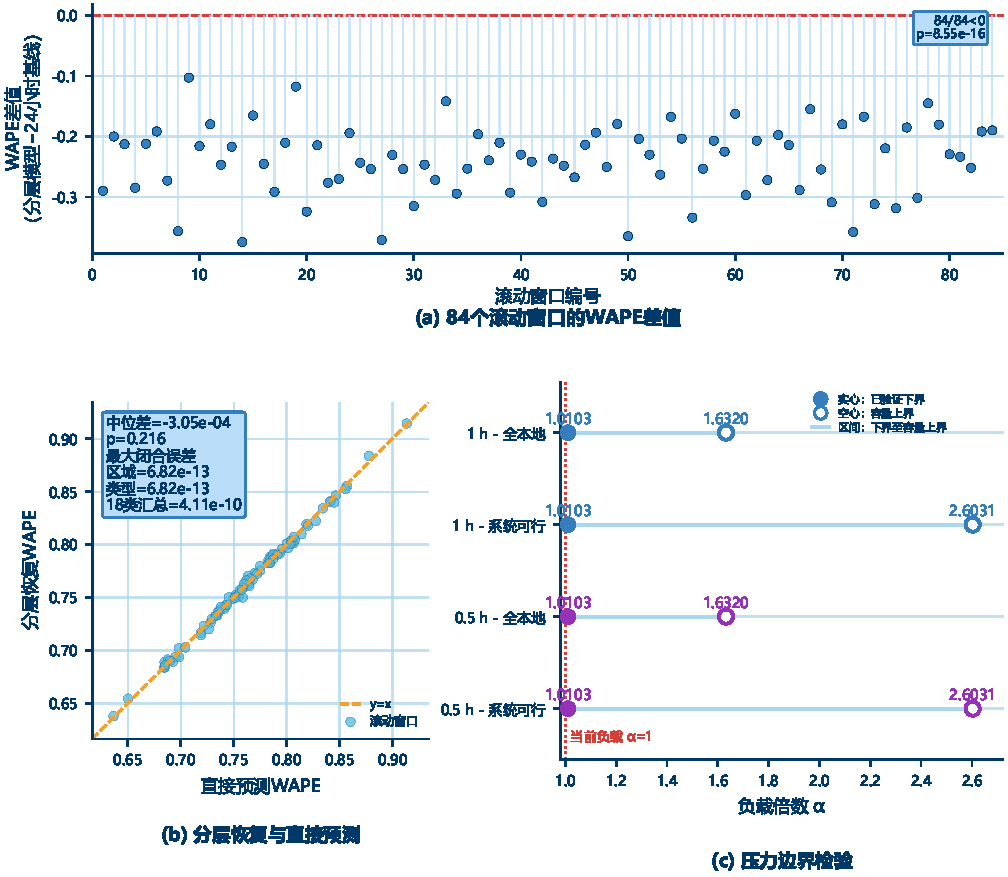
\includegraphics[width=0.91\textwidth]{figures/q1_group3_validation_robustness.pdf}
%	\caption{分层预测稳定性与算力调度压力边界检验}
%\end{figure}
%% =================================================
%
%除预测稳定性外，还对基础调度的资源边界进行了压力检验。
%设原始任务负荷按照比例系数$\alpha$整体放大，
%当前运行点对应$\alpha=1$。
%图3(c)表明，已经实际验证可行的负载下界为$\alpha=1.0103$；
%在容量关系下，保持全本地运行的上界为1.6320，
%允许跨区域协调后的系统容量上界为2.6031。
%需要强调的是，1.6320和2.6031仅表示由资源容量关系得到的上界，
%并不能直接解释为已经验证可行的精确临界负载。
%因此，该压力测试更准确地给出了
%“已验证可行负荷”与“理论容量上限”之间的边界区间。
%
%此外，为检验整数小时开工假设是否影响核心调度结论，
%进一步采用0.5小时粒度重新求解。
%1小时和0.5小时两种粒度下均得到
%$F_1^*=0$，
%说明“当前任务无需跨区域迁移”这一一级结论保持不变；
%累计弹性等待时间则由3 h下降至2 h，
%表明时间粒度细化主要改善少量任务的局部开工安排，
%并未改变整体空间调度判断。
%与此同时，对任务唯一执行、实时任务立即启动、网络时延、
%最早开工、最晚完成、2406终端边界以及GPU、IT功率和设施功率等硬约束进行复核，
%均未发现约束违反。
%
%综合上述结果，
%问题一的分层预测能够在保留区域与任务类型异质性的同时，
%稳定提取短期GPU需求水平；
%层级一致性恢复在几乎不改变预测精度的情况下保证了多层需求闭合。
%基础算力调度则表明，
%当前任务规模下六区域已有资源能够支持全部任务本地完成，
%但不同区域的GPU、AI IT功率和设施功率瓶颈存在明显差异。
%这些结果为后续碳感知调度提供了明确基线：
%后续产生的跨区域迁移应主要反映电价、碳强度和新能源条件所带来的算电协同效应。
%
\section{问题一的模型建立与求解}

\subsection{数据预处理}

原始数据含50000个任务、6个区域和3类任务，到达时刻覆盖第0--2399小时。检查字段完整性与取值范围后，将持续时间由分钟换算为小时，按任务类型匹配单位GPU功率，并按最大网络时延筛选候选区域；各物理量不作标准化或异常值删除。预测数据按“到达小时--来源区域--任务类型”聚合并补齐零需求，共43200条记录；第0--2351小时用于训练，第2352--2375小时用于验证，第2376--2399小时用于测试。调度直接采用测试期实际任务，第2400--2405小时用于收尾，第2406小时为终端边界。


\subsection{模型建立}

问题一分别进行GPU需求短期预测与基础算力调度，预测结果仅用于精度评价，不参与实际调度。

设区域$r$、任务类型$k$在时刻$t$的新到达GPU需求为$D_{rkt}$，
任务$i$的GPU需求为$g_i$，则
\begin{equation}
	D_{rkt}
	=
	\sum_{\substack{i:\,a_i=t\\
			r_i^0=r,\;k(i)=k}}
	g_i .
	\label{eq:q1_demand}
\end{equation}

由此得到18条底层序列，并构造区域需求$D_{rt}=\sum_kD_{rkt}$、任务类型需求$D_{kt}=\sum_rD_{rkt}$和系统需求$D_t=\sum_rD_{rt}$。底层序列保留异质性，三个聚合层用于提高短期预测稳定性。

层级与分组时间序列需通过预测协调保持层间一致\cite{ref4}。本文以历史业务占比构造非负先验，采用广义KL散度恢复18类交叉需求，借鉴一致性恢复思想而不直接使用Trace MinT目标函数。

对于任一聚合需求序列$y_t$，
采用预测时点前最近$H$小时的平均需求水平预测未来24小时：
\begin{equation}
	\hat{y}_{T+h}(H)
	=
	\frac{1}{H}
	\sum_{\tau=T-H+1}^{T}y_{\tau},
	\qquad h=1,2,\ldots,24 .
	\label{eq:q1_localmean}
\end{equation}

其中$T$为预测前最后一个已知时刻。由验证集在$H\in\{24,72,168,336\}$中选窗，再用第0--2375小时信息预测第2376--2399小时，测试期不参与模型选择。

区域、任务类型和系统需求分别预测后可能出现总量不一致，
因此首先以系统预测$\hat D_t^{(S)}$作为总量锚点，
对区域和任务类型边际进行比例校正，
得到$\tilde D_{rt}$和$\tilde D_{kt}$。
设历史区域--任务类型平均需求占比为$q_{rk}$，
构造与GPU需求同量纲的先验
$q^0_{rkt}=q_{rk}\hat D_t^{(S)}$；
对于历史占比为0的组合赋予极小正数以避免对数奇异。
随后利用广义KL散度恢复18类交叉需求：
\begin{equation}
	\begin{aligned}
		\min_{z_{rkt}\geq0}\quad
		&\sum_r\sum_k
		\left[
		z_{rkt}\ln\frac{z_{rkt}}{q^0_{rkt}}
		-z_{rkt}+q^0_{rkt}
		\right],\\
		\mathrm{s.t.}\quad
		&\sum_kz_{rkt}=\tilde D_{rt},\\
		&\sum_rz_{rkt}=\tilde D_{kt}.
	\end{aligned}
	\label{eq:q1_kl}
\end{equation}

式(\ref{eq:q1_kl})在保持两类边际不变时使18类需求接近历史结构。预测采用WAPE、RMSE和MAE评价，以24小时前同刻需求为基准。

基础算力调度直接采用第2376--2399小时实际到达任务。
设任务$i$持续时间为$d_i$、来源区域为$r_i^0$，
根据网络时延确定候选区域$R_i$。
实时推理任务到达即开工；
批量推理和AI训练任务在最早开工时间、最晚完成时间及2406终端边界内确定候选开工集合$S_i$。
定义$x_{irs}$表示任务$i$是否在区域$r$、时刻$s$开工。

由于任务持续时间保留分钟精度，而资源容量按小时统计，
定义任务$i$从时刻$s$开始后与小时区间$[t,t+1)$的实际运行比例为
\begin{equation}
	\rho_{ist}
	=
	\max\left\{
	0,\,
	\min(s+d_i,t+1)-\max(s,t)
	\right\}.
	\label{eq:q1_overlap}
\end{equation}

由式(\ref{eq:q1_overlap})可计算逐小时GPU和功率占用。
任务$i$完整运行时的AI IT功率为
$p_i=g_iP^{GPU}_{k(i)}$。
区域$r$在时刻$t$可供AI任务使用的有效IT功率定义为
\[
A_{rt}
=
\max\left\{
0,\,
\min\left(
P^{IT,\max}_r-P^{NonAI}_{rt},
\frac{P^{Facility,\max}_r}{PUE_r}-P^{NonAI}_{rt}
\right)
\right\}.
\]
主要资源约束为
\begin{equation}
	\begin{aligned}
		&\sum_{r\in R_i}\sum_{s\in S_i}x_{irs}=1,
		&&\forall i,\\
		&\sum_i\sum_{s\in S_i}
		g_i\rho_{ist}x_{irs}
		\leq G^{ava}_{rt},
		&&\forall r,t,\\
		&\sum_i\sum_{s\in S_i}
		p_i\rho_{ist}x_{irs}
		\leq A_{rt},
		&&\forall r,t .
	\end{aligned}
	\label{eq:q1_capacity}
\end{equation}

式(\ref{eq:q1_capacity})保证任务唯一执行及GPU、功率容量可行；$R_i$和$S_i$预先筛除违反时延、时窗或终端边界的组合。

问题一不引入电价、碳排放、新能源和储能因素，
因此作为后续算电协同调度的中性算力基线。
首先最小化跨区域迁移GPU工作量，
再在一级目标最优的条件下最小化弹性任务累计等待时间：
\begin{equation}
	\begin{aligned}
		\min\quad
		F_1
		&=
		\sum_i
		\sum_{\substack{r\in R_i\\r\neq r_i^0}}
		\sum_{s\in S_i}
		g_id_ix_{irs},\\
		\text{在 }F_1=F_1^{*}\text{ 条件下，}\qquad
		\min\quad
		F_2
		&=
		\sum_{i\in I^{\mathrm{flex}}}
		\sum_{r\in R_i}\sum_{s\in S_i}
		(s-e_i)x_{irs}.
	\end{aligned}
	\label{eq:q1_objective}
\end{equation}

其中$F_1$衡量迁移GPU工作量，$F_2$为弹性任务累计等待时间。


\subsection{求解结果与模型检验}

验证集中$H=72$的总体WAPE最低，据此用第0--2375小时历史数据预测第2376--2399小时的18类GPU需求。

RegionD、RegionE和RegionF的AI训练累计GPU需求分别为
407683、292000和296143，
明显高于RegionA、RegionB和RegionC的
63070、62551和58899；
同时底层小时需求存在较多低值和随机尖峰，
说明直接预测18条细粒度序列容易受到随机任务到达影响。

% ==================== Q1：预测误差对比 ====================
\begin{table}[H]
	\centering
	\caption{分层预测模型与24小时同刻基准误差对比}
	\label{tab:q1_forecast}
	
	\fontsize{10.5pt}{12pt}\selectfont
	\renewcommand{\arraystretch}{0.88}
	
	\begin{tabular}{ccccccc}
		\toprule
		\multirow{2}{*}{\textbf{阶段}}
		& \multicolumn{3}{c}{\textbf{分层局部均值预测}}
		& \multicolumn{3}{c}{\textbf{24小时同刻基准}}\\
		\cmidrule(lr){2-4}\cmidrule(lr){5-7}
		& \textbf{WAPE} & \textbf{RMSE} & \textbf{MAE}
		& \textbf{WAPE} & \textbf{RMSE} & \textbf{MAE}\\
		\midrule
		验证期
		& 0.7241 & 45.7417 & 23.6915
		& 1.0957 & 69.9249 & 35.8495\\
		
		测试期
		& 0.6519 & 53.4704 & 26.3323
		& 0.8740 & 72.8628 & 35.3032\\
		\bottomrule
	\end{tabular}
\end{table}


表\ref{tab:q1_forecast}中，分层模型在验证期和测试期的三项误差均低于24小时同刻基准。题面分别要求短期需求预测和末段基础算力调度，因此预测结果用于评价需求变化的可预测程度，实际调度仍以第2376--2399小时真实到达的任务为输入，避免预测误差改变任务级可行性。验证期与测试期的WAPE分别为0.7241和0.6519，表明稀疏需求和随机尖峰仍较难准确刻画。测试期WAPE降低而RMSE升高并不矛盾：WAPE按总实际需求归一化，RMSE则对少数较大误差更加敏感，二者反映了不同的误差特征。

\begin{figure}[H]
	\centering
	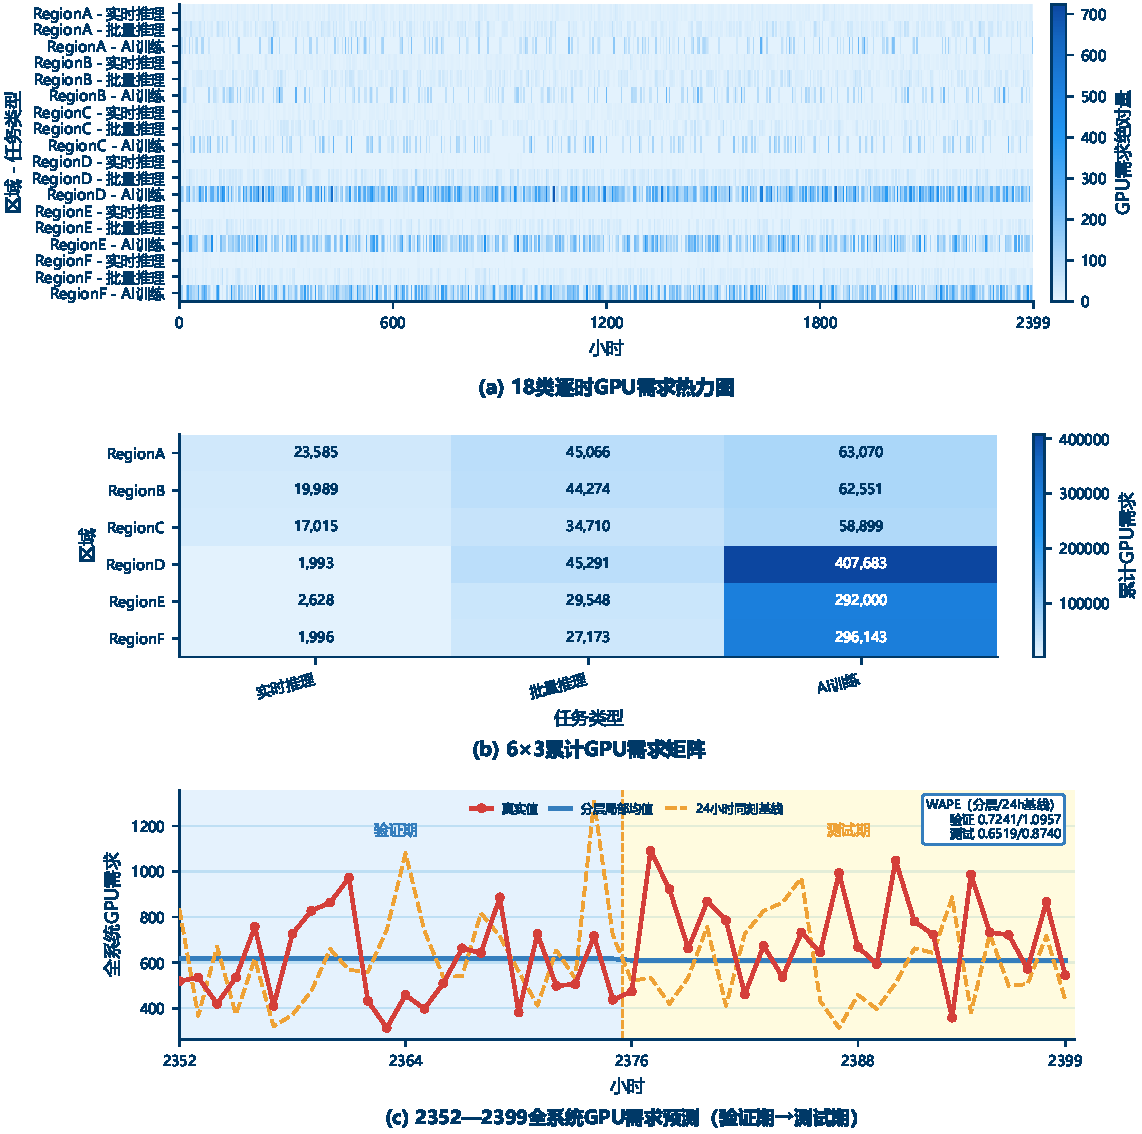
\includegraphics[width=0.80\textwidth]{figures/q1_group1_demand_structure.pdf}
	\caption{GPU需求异质性与分层短期预测结果}
	\label{fig:q1_forecast}
\end{figure}

图\ref{fig:q1_forecast}显示模型主要刻画短期需求水平，不追踪随机单小时尖峰。

基础调度对第2376--2399小时实际到达的538个任务按式(\ref{eq:q1_objective})进行两级优化。

% ==================== Q1：基础调度结果 ====================
\begin{table}[H]
	\centering
	\caption{基础算力调度优化结果}
	\label{tab:q1_dispatch}
	
	\fontsize{10.5pt}{12pt}\selectfont
	\renewcommand{\arraystretch}{0.88}
	
	\begin{tabular}{cc}
		\toprule
		\textbf{评价指标} & \textbf{优化结果}\\
		\midrule
		任务数量 & 538\\
		一级目标$F_1^*$ & $0$ GPU$\cdot$h\\
		本地执行率 & 100\%\\
		二级目标$F_2^*$ & 3 h\\
		求解相对间隙 & 0\\
		\bottomrule
	\end{tabular}
\end{table}


表\ref{tab:q1_dispatch}中$F_1^*=0$、$F_2^*=3$ h，538个任务均可在来源区域完成，当前资源下无须迁移即可保证可行。

\begin{figure}[H]
	\centering
	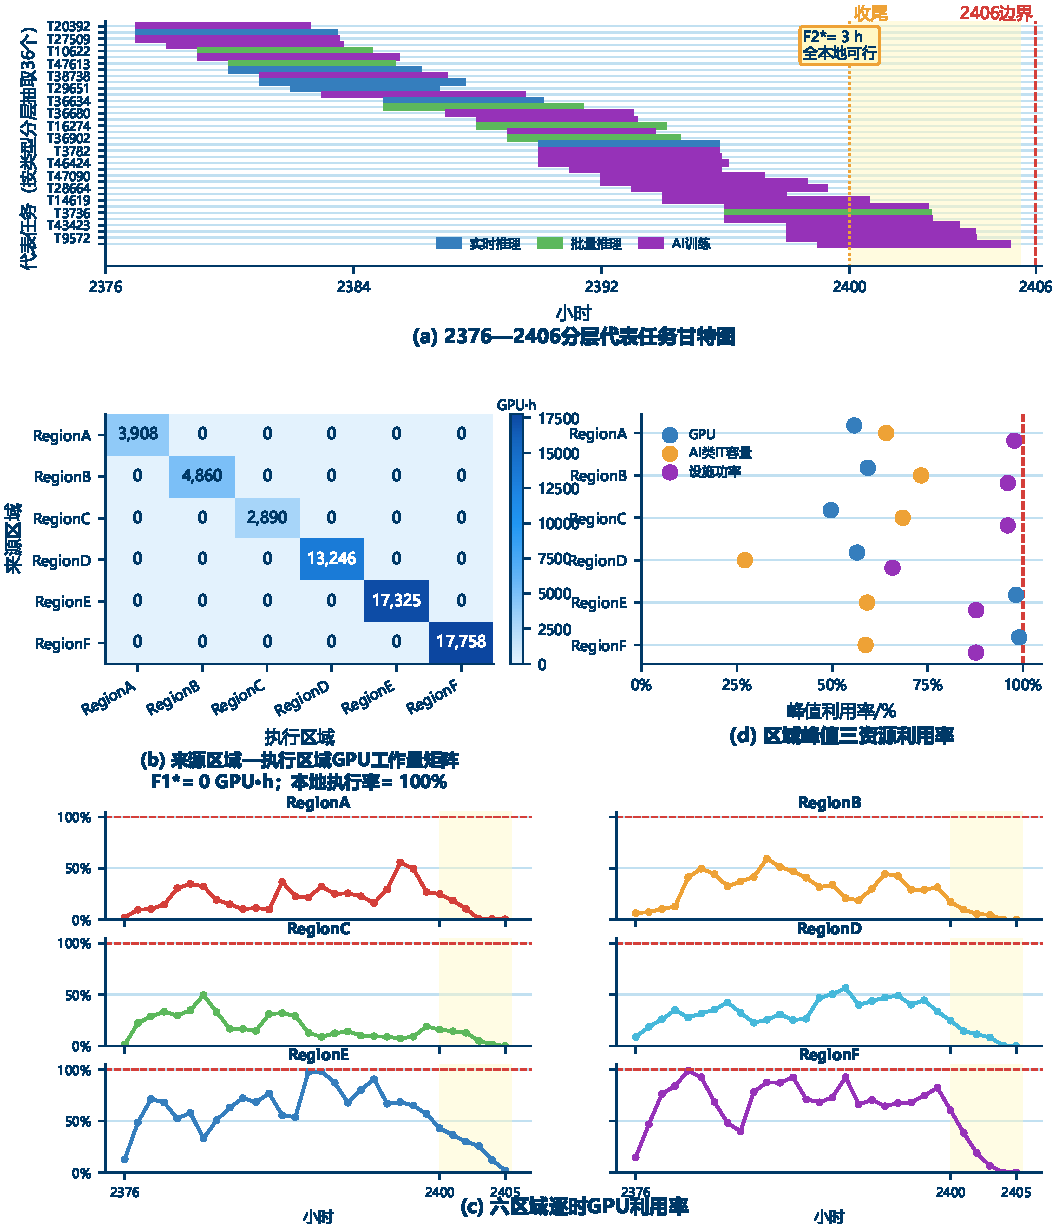
\includegraphics[width=0.75\textwidth]{figures/q1_group2_core_results.pdf}
	\caption{基础算力调度方案与多资源承载状态}
	\label{fig:q1_dispatch}
\end{figure}

图\ref{fig:q1_dispatch}显示，末端任务均在2406前完成，区域间GPU工作量矩阵仅主对角线非零；RegionE、RegionF部分时段接近GPU容量边界，部分东部区域受设施功率限制。

84个滚动样本外窗口中，分层模型WAPE均低于24小时同刻基准；单侧Wilcoxon检验得$p=8.55\times10^{-16}$。

一致性恢复与直接预测的WAPE中位差为$-3.05\times10^{-4}$（$p=0.216$），区域、类型边际最大闭合误差均为$6.82\times10^{-13}$，18类汇总误差为$4.11\times10^{-10}$。其作用是保证多层预测闭合，而非提高精度。

\begin{figure}[H]
	\centering
	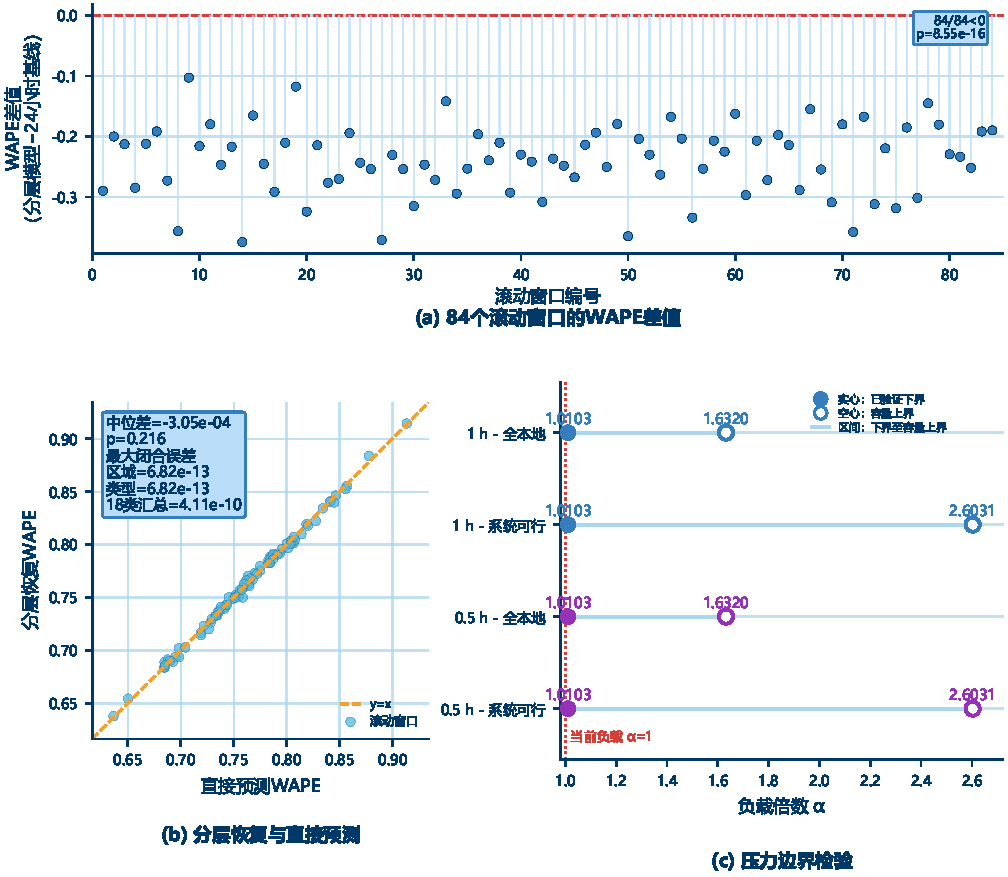
\includegraphics[width=0.80\textwidth]{figures/q1_group3_validation_robustness.pdf}
	\caption{分层预测稳定性与算力调度压力边界检验}
	\label{fig:q1_validation}
\end{figure}

图\ref{fig:q1_validation}中，负荷放大系数$\alpha$的已验证可行下界为1.0103；全本地和跨区域协调的容量理论上界分别为1.6320、2.6031，后两者并非已验证的精确临界值。

0.5小时粒度复算仍有$F_1^*=0$，累计等待由3 h降至2 h，未改变无需迁移的结论；任务唯一执行、实时启动、时延、时限及各容量约束均未发现违反。

问题一由此形成短期需求预测和纯算力调度基准，供问题二引入能源因素后比较。


